\chapter{Introduction}
\thispagestyle{empty}

\begin{itemize}
    \item \textcolor{red}{Background}
    \item \textcolor{red}{Galaxy Evolution}
    \item \textcolor{red}{Galaxy Distribution}
    \item \textcolor{red}{Star-Forming Galaxies}
    \item \textcolor{red}{Black Holes}
    \item \textcolor{red}{Active Galactic Nuclei}
    \item \textcolor{red}{Feedback Mechanisms}
    \item \textcolor{red}{Cosmic Evolution and Conclusion}
\end{itemize}

\section{Galaxy Evolution}
The simple distribution of galaxies and their luminosities have previously derived powerful constraints on galaxy evolution \citep{biviano_spitzer_2011} \textcolor{red}{(more citations?)}. One of the direct ways of measuring the distribution of galaxies is with the luminosity function \citep{schechter_analytic_1976, saunders_60-mum_1990}. Luminosity functions (LF) are statistical distributions that describe the spatial density of astronomical objects and are a fundamental tool for quantifying their evolution across cosmic time scales \citep{dai_mid-infrared_2009, han_evolution_2012, wylezalek_galaxy_2014}. The use of LFs in galaxy evolution studies has uncovered a wealth of information revealing the intricate processes governing star formation, galaxy mergers, and the growth of supermassive black holes (SMBH, $M_{BH} > 10^{6} M_{\odot}$) across cosmic time \citep{caputi_infrared_2007, hopkins_observational_2007, rodighiero_mid-_2010, gruppioni_modelling_2011, gruppioni_herschel_2013, magnelli_deepest_2013, delvecchio_tracing_2014, hernan-caballero_resolving_2015, symeonidis_agn_2021, thorne_deep_2022}. Specifically, many such studies find a strong correlation between the activity of the central SMBH and the star formation rate (SFR) \citep{hopkins_cosmological_2008, merloni_synthesis_2008}. 

\begin{figure}[t!]
    \setlength{\abovecaptionskip}{60pt} % Extra white space for video player
    \embedvideo*{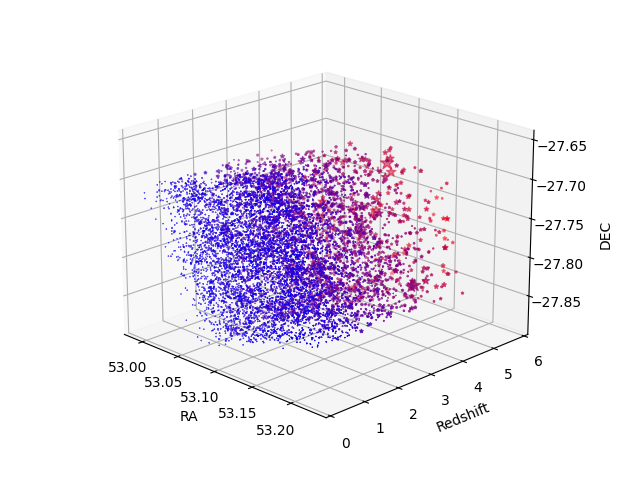
\includegraphics[width=\textwidth]{Figures/CDFS}}{Figures/CDFS.mp4}
    \caption{Animated 3D-view of ZFOURGE CDFS field galaxies coloured by redshift.}
    \setlength{\abovecaptionskip}{10pt} % Reset to default
\end{figure}